%!TEX TS-program = pdflatex

\documentclass[aspectratio=169]{beamer}

%packages
\usepackage{amsmath,amsthm,amssymb,amsfonts,amsxtra,amstext}
\usepackage{graphicx,float}
\usepackage{media9} %needed for including movies, otherwise comment out
%various figure appearance tweaks:
\usepackage{subcaption}
\captionsetup[subfigure]{labelformat=empty,margin=1ex,justification=raggedright}
\captionsetup[figure]{labelformat=empty}
%table tweaks
\usepackage{multirow}
\usepackage{multicol}
%tikz stuff - can be safely commented out if not using tikz for anything
\usepackage{tikz}
\usetikzlibrary{tikzmark,fit,shapes.geometric,positioning,arrows,arrows.meta}
\tikzstyle{every picture}+=[remember picture]
\usepackage{animate}

%add your own graphics path as needed:
%\graphicspath{{../Common/Figures/}{../Common/Logos/}}

%presentation theme and Cornell branding
\usetheme{Frankfurt} %if you don't like the navigation links up top, switch to: \usetheme[]{Madrid}
\DefineNamedColor{named}{CornellRed}{cmyk}{0,1,0.79,0.2} 
\usecolortheme[named=CornellRed]{structure}
\usefonttheme[]{serif}
\setbeamertemplate{navigation symbols}{} %i find these useless. ymmv

%logos
\pgfdeclareimage[height=1.5cm]{culogo}{template/CULogored}
\pgfdeclareimage[height=0.625cm]{CULogowhite}{template/CULogowhite}
\pgfdeclareimage[height=1.5cm]{csilogo}{template/CSI_logo}
\pgfdeclareimage[height=1.5cm]{sioslogo}{template/SIOSLogo_color_vector}

%let's slap the Cornell logo on everything. branding!
\usepackage[absolute,overlay]{textpos}
\setlength{\TPHorizModule}{1mm}
\setlength{\TPVertModule}{1mm}
\newcommand{\MyLogo}{%
\begin{textblock}{14}(153.0,6.35)
  \pgfuseimage{CULogowhite}
\end{textblock}
}

%\BackgroundPicture creates a full-slide image 
%see below for usage example
\newcommand\BackgroundPicture[3]{%
    \setbeamertemplate{background}{%
    \parbox[c][\paperheight]{\paperwidth}{%
        %\vfill \hfill
 \includegraphics[width=#2\paperwidth,height=#3\paperheight]{#1}
         %\hfill \vfill
      }}}


%useful defs - add your own here
\def\mf{\mathbf}
\def\mb{\mathbb}
\def\mc{\mathcal}
\newcommand{\mfbar}[1]{\mf{\bar{#1}}}
\newcommand{\mfhat}[1]{\mf{\hat{#1}}}
\newcommand{\bdot}[1]{\ensuremath{\dot{\mathbf{#1}}}}
\newcommand{\bhat}[1]{\ensuremath{\hat{\mathbf{#1}}}}
\newcommand{\intd}[1]{\ensuremath{\,\mathrm{d}#1}}
\newcommand{\leftexp}[2]{{\vphantom{#2}}^{#1}\!{#2}}
\newcommand{\leftsub}[2]{{\vphantom{#2}}_{#1}\!{#2}}
\newcommand{\fddt}[1]{\ensuremath{\leftexp{\mathcal{#1}}{\frac{\mathrm{d}}{\mathrm{d}t}}}}
\newcommand{\fdddt}[1]{\ensuremath{\leftexp{\mathcal{#1}}{\frac{\mathrm{d}^2}{\mathrm{d}t^2}}}}
\newcommand{\omegarot}[2]{\ensuremath{\leftexp{\mathcal{#1}}{\boldsymbol{\omega}}^{\mathcal{#2}}}}
\newcommand{\refeq}[1]{Equation  (\ref{#1})} 
\newcommand{\reftable}[1]{Table \ref{#1}}  
\newcommand{\reffig}[1]{Figure \ref{#1}}
\newcommand{\refnum}[1]{Ref.~\citenum{#1}}

%fonts and colors - add own defs here
\setbeamerfont{smalleq}{size=\tiny} 
\definecolor{MyBlue}{cmyk}{0.88, 0.7637,0.0032,0} 
\definecolor{MyRed}{cmyk}{0,0.994,1,0} 
\definecolor{MyGreen}{cmyk}{0.8985,0.3258,1,0.2429} 
\definecolor{MyPurple}{cmyk}{0.7708,0.847,0,0} 
\definecolor{MyGraphite}{cmyk}{0.5973,0.5124,0.5077,0.2013} 

% presentation descriptors
\title[]{Scheduling Direct Imaging Observations of Exoplanets Based on Radial Velocity Data}
\subtitle[]{Best Practices and Failure Modes}
\author[]{Corey Spohn}
%if you don't want logos on the title page (or don't want all of them, modify this:
\institute[]{\pgfuseimage{culogo}\hspace{0.75cm}\pgfuseimage{csilogo}\hspace{0.75cm}\pgfuseimage{sioslogo}}
\date[]{10/13/2021}
\subject{Talks} %modify as desired

%bib stuff 
%\usepackage[backend=biber, style=authoryear-comp]{biblatex}
\usepackage[style=authoryear]{biblatex}
\addbibresource{library.bib} %change to your own bibliography file

%custom cite command - change at will (change tiny to footnotesize to make bigger)
\newcommand{\customcite}[1]{\tiny{\citeauthor{#1}, \citetitle{#1}, \citeyear{#1}}}
\newcommand{\customcitenorm}[1]{{\citeauthor{#1}, \citetitle{#1}, \citeyear{#1}}}

% add a macro that saves its argument
\makeatletter
\newcommand{\footlineextra}[1]{\gdef\insertfootlineextra{#1}}
\newbox\footlineextrabox

% add a beamer template that sets the saved argument in a box.
% The * means that the beamer font and color "footline extra" are automatically added. 
\defbeamertemplate*{footline extra}{default}{
    \begin{beamercolorbox}[ht=2.25ex,dp=1ex,leftskip=1ex,wd=0.95\paperwidth]{footline extra}
    \insertfootlineextra
    %\par\vspace{2.5pt}
    \end{beamercolorbox}
}

\addtobeamertemplate{footline}{%
    % set the box with the extra footline material but make it add no vertical space
    \setbox\footlineextrabox=\vbox{\usebeamertemplate*{footline extra}}
    \vskip -\ht\footlineextrabox
    \vskip -\dp\footlineextrabox
    \box\footlineextrabox%
}

% patch \begin{frame} to reset the footline extra material
\let\beamer@original@frame=\frame
\def\frame{\gdef\insertfootlineextra{}\beamer@original@frame}
\footlineextra{}
\makeatother

%record left margin for making things full-frame
\makeatletter
\newlength\beamerleftmargin
\setlength\beamerleftmargin{\Gm@lmargin}
\makeatother
\graphicspath{{./}{figures/}}

\beamertemplategridbackground[10pt]

% TikZ stuff
\tikzset{
  every overlay node/.style={
    draw=black,fill=white,anchor=north west,inner sep=0, outer sep=0,
  },
}
% Usage:
% \tikzoverlay at (-1cm,-5cm) {content};
% or
% \tikzoverlay[text width=5cm] at (-1cm,-5cm) {content};
\def\tikzoverlay{%
   \tikz[baseline,overlay]\node[every overlay node]
}%


\begin{document}

\part{Talk}
\frame[plain]{\titlepage
\vfill
\centering
%{\tiny You may wish to put auspices statements here, or not}
}

%after the title page, set up slide appearance
\setbeamertemplate{background}{ \setbeamercolor{normal text}{bg=white} }
\addtobeamertemplate{headline}{}{\MyLogo}
\setbeamertemplate{navigation symbols}{\insertframenumber{}/\inserttotalframenumber}
\beamertemplategridbackground[1cm]

\section{Introduction}
\subsection{Introduction} %note that you need both sections and subsection for the navigation to look good for this 

%here's a normal slide:
\frame{
\frametitle{Exoplanet exploration}
\tikzoverlay[text width = 8cm] at (0cm, 3cm+4.5pt){
\begin{itemize}
    \item  NASA's Exoplanet Exploration Program's primary goal is to ``discover and characterize
        planetary systems and Earth-like planets around nearby stars''
    \item Further, the program is looking for signs of possible life which is studied through
        atmospheric characterization
    \item To make detailed atmospheric characterization we need light from an exoplanet, either via
        transmission spectroscopy or direct imaging.
\end{itemize}
};
\tikzoverlay[text width = 5cm] at (8.35cm, 1.65cm){
    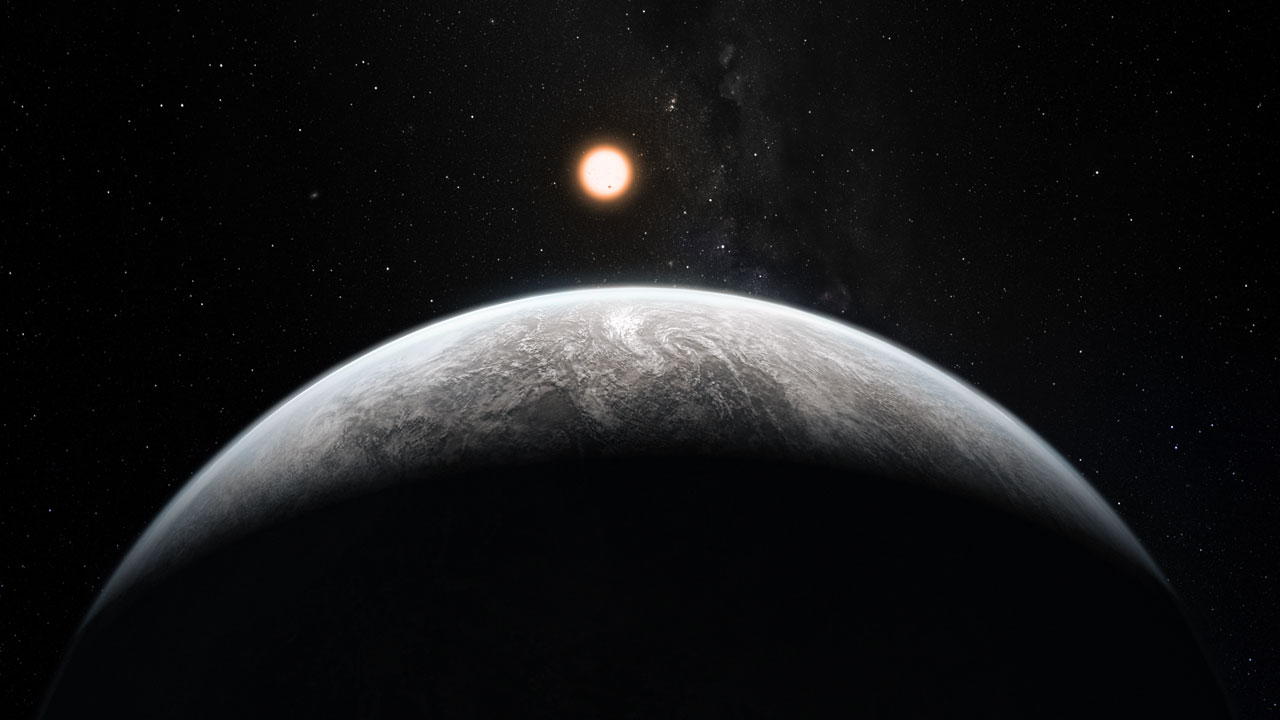
\includegraphics[width=6cm]{figures/exoplanet_art.jpeg}
};
\footlineextra{https://exoplanets.nasa.gov/system/internal\_resources/details/original/852\_Super\_Earth.jpeg}
}

\frame{
\frametitle{Direct Imaging}
\tikzoverlay[text width = 14cm] at (0cm, 3cm+4.5pt){
\begin{itemize}
    \item  Detecting a planet as a point source of light
    %\item Sensitive to a different population of planets than indirect detection methods
    \item Technical challenge, researching many different ways to increase the number of planets we
        detect
\end{itemize}
};
\tikzoverlay[text width = 8cm] at (2cm-3pt, 4.5pt+1cm){
    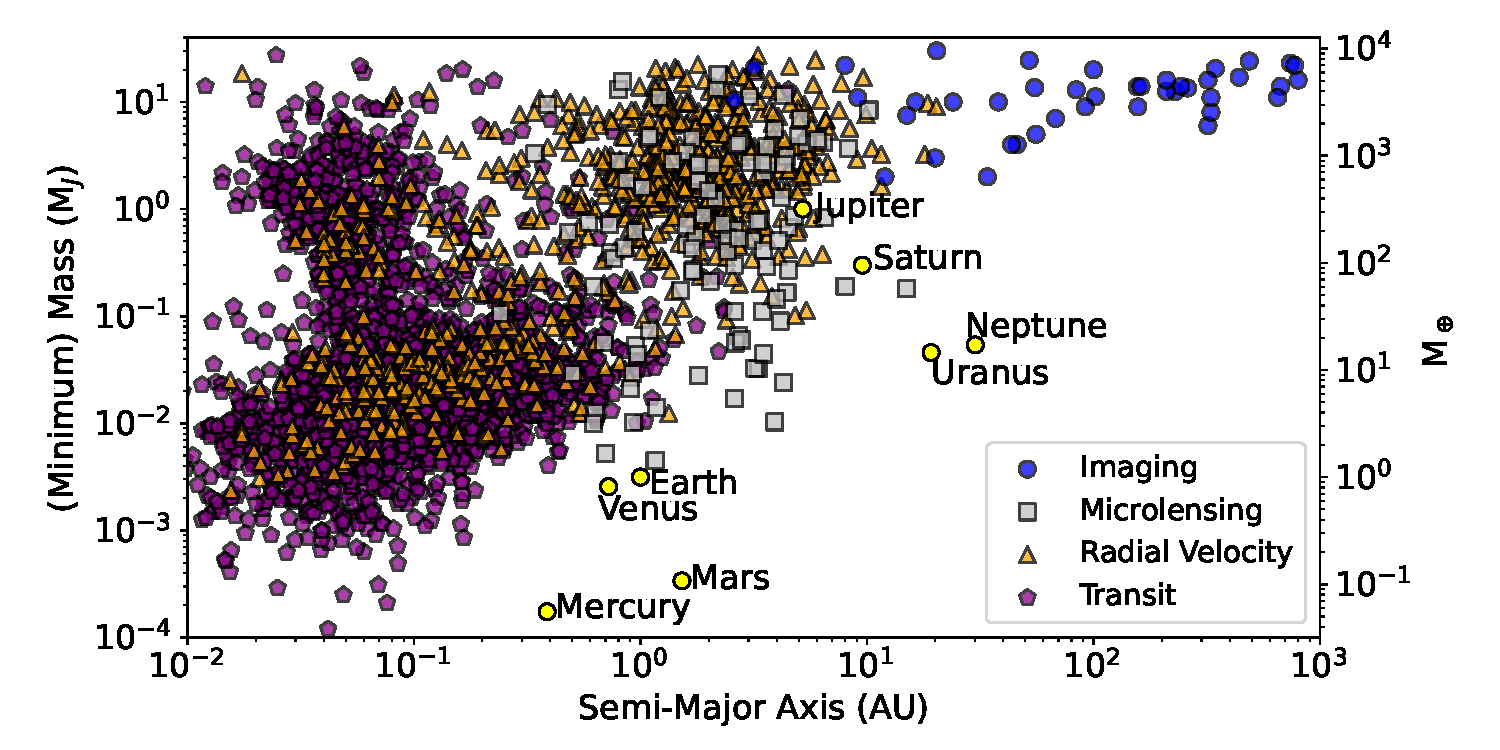
\includegraphics[width=10cm]{figures/all_planets.pdf}
};
%\tikzoverlay[text width = 5cm] at (8.35cm, 1.65cm){
    %\animategraphics[loop, controls, width=4cm]{5}{HR_8799_gif/HR_8799-}{0}{100}
%};
}

\frame{
\frametitle{Ways to image more exoplanets}
\tikzoverlay[text width = 14cm] at (0cm, 3cm+4.5pt){
\begin{itemize}
    \item Improve instruments
    \item Use the limited observation time more effectively
\end{itemize}
};
\tikzoverlay[text width = 3cm] at (4.5cm-3pt, 1.5cm+4.5pt){
    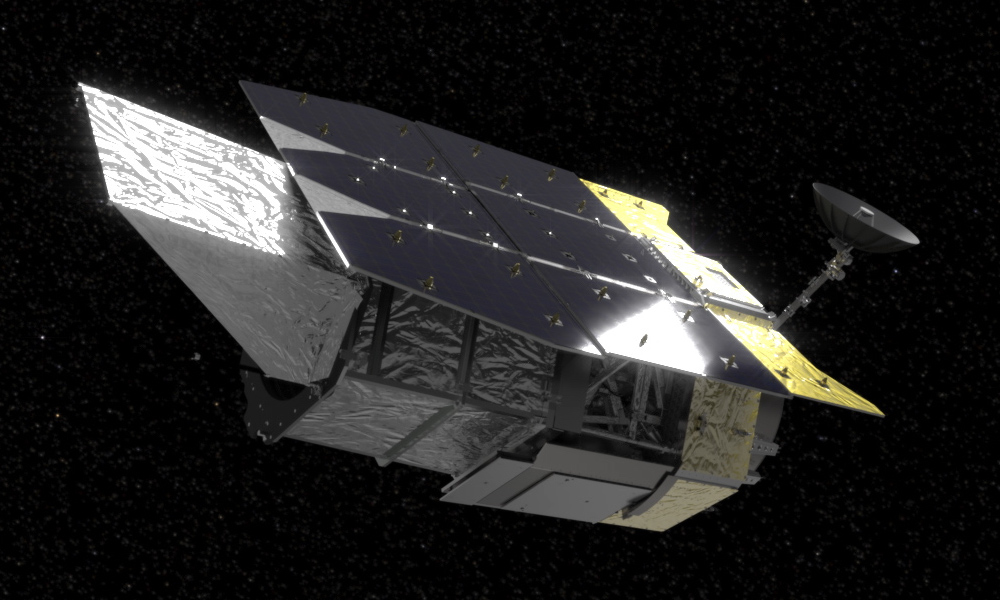
\includegraphics[height=3cm]{figures/roman_space_telescope.jpg}
};
\tikzoverlay[text width = 10cm] at (2cm-7pt, -1.5cm+4.5pt){
    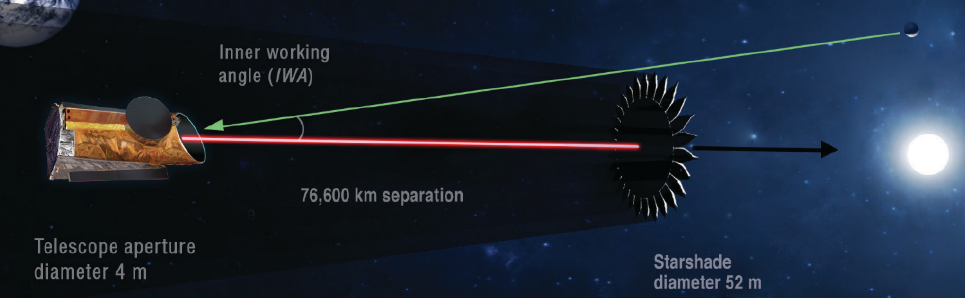
\includegraphics[width=10cm]{figures/habex.png}
};
}

\frame{
    \frametitle{Precursor radial velocity detections}
\tikzoverlay[text width = 14cm] at (0cm, 3cm+4.5pt){
\begin{itemize}
    \item Detect planets ahead of time via the radial velocity method
    \item Currently being used by the Nancy Grace Roman Space Telescope team to identify exoplanet targets
    \item The HabEx team notes ``Precise precursor radial velocities (PRVs) will
        provide multiple advantageous contributions to the scientific yield and optimization of
        HabEx.''\parencite{HabEx2020}
\end{itemize}
};
\tikzoverlay[text width = 6cm] at (0cm-2pt, -0.4cm+4.5pt){
    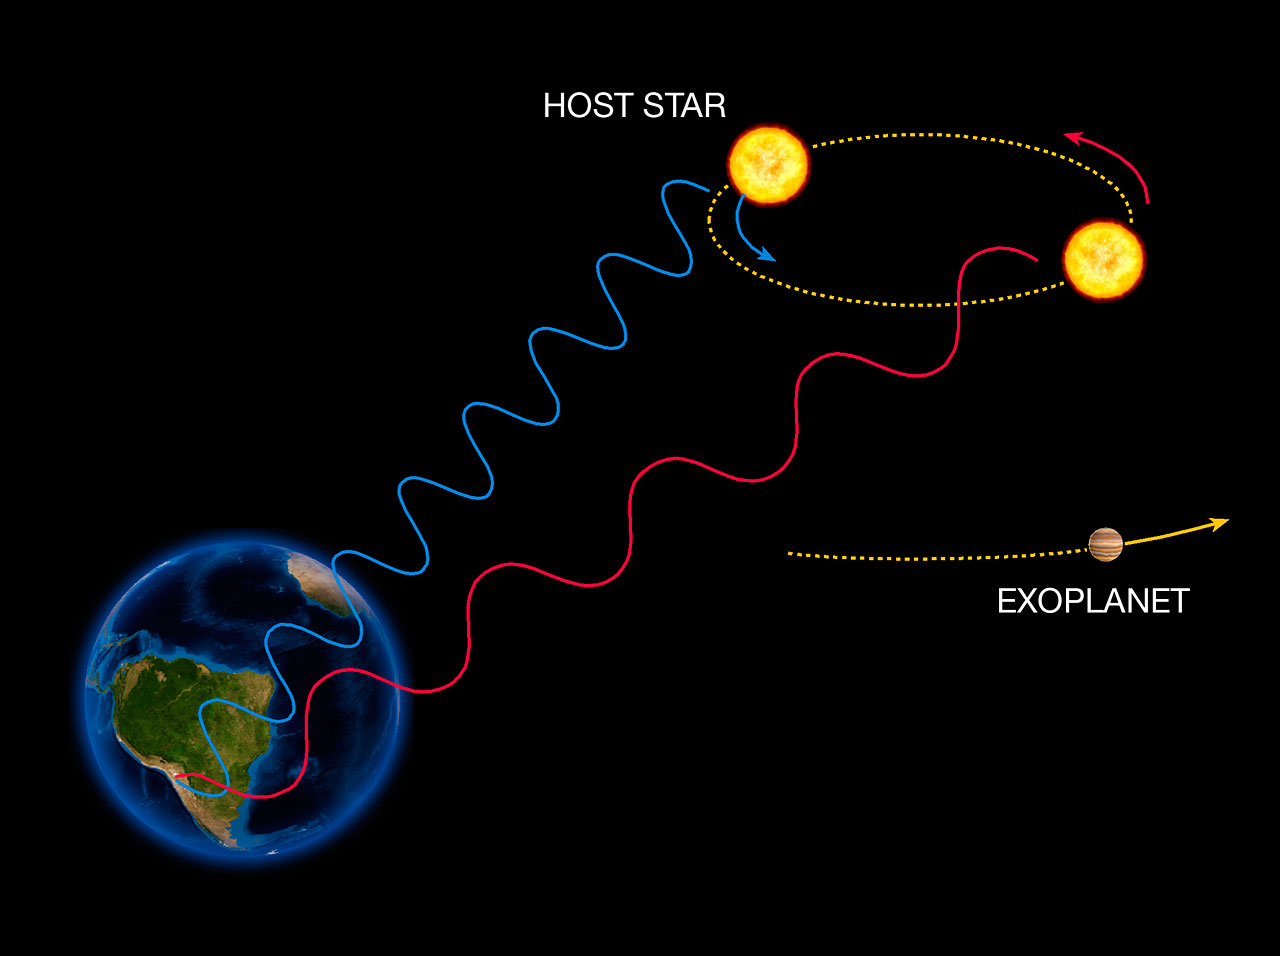
\includegraphics[height=3.75cm]{figures/RV_method_art.jpg}
};
\tikzoverlay[text width = 6cm] at (6cm, -0.4cm+4.5pt){
    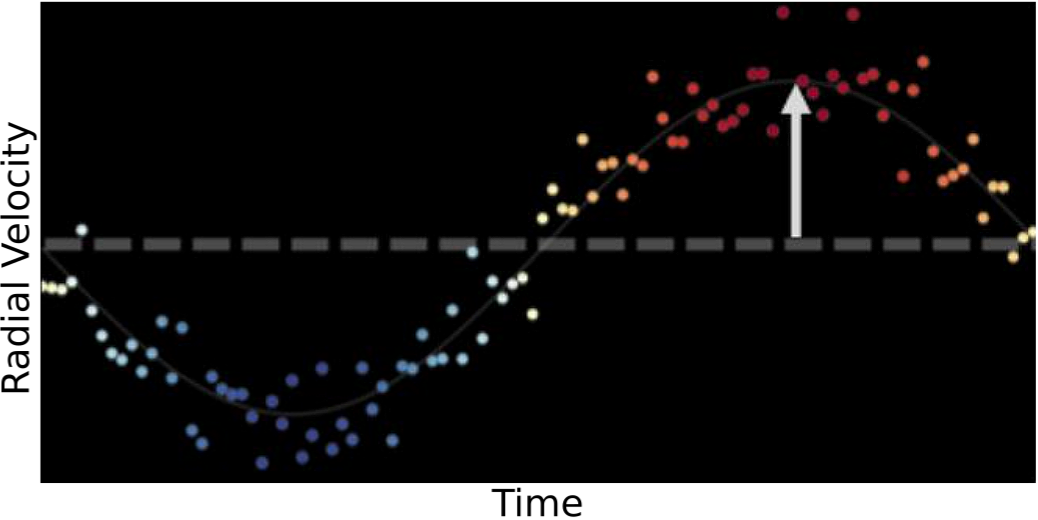
\includegraphics[height=3.75cm]{figures/export2.png}
};
%TODO FIX SECOND PICTURE
\footlineextra{ESO, \textcite{EPRV2020}}
}

\frame{
    \frametitle{Current radial velocity precision}
\tikzoverlay[text width = 14cm] at (0cm, -2.8cm+4.5pt){
\begin{itemize}
    \item Need approximately 10 cm/s precision to detect Earth-like planets
    \item Predicting detectability based on precision RV data
\end{itemize}
};
\tikzoverlay[text width = 6cm] at (2cm, 3cm+4.5pt){
    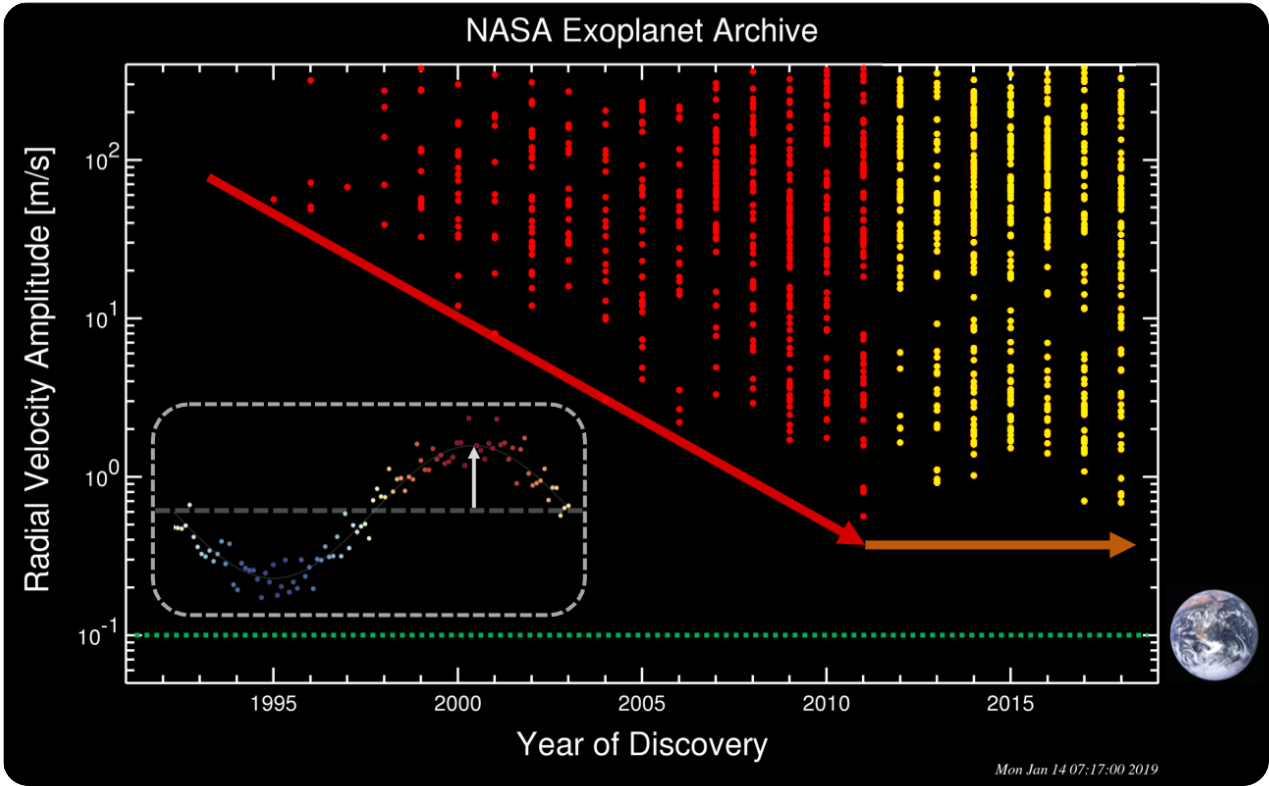
\includegraphics[height=6cm]{figures/RV_precision.png}
};
\footlineextra{\textcite{EPRV2020} }
}

\frame{
    \frametitle{Mass/inclination ambiguity}
\tikzoverlay[text width = 6cm] at (1cm, 3cm+4.5pt){
    \animategraphics[loop, controls, width=12cm]{10}{mass_inclination_comparision/frame-}{0}{99}
};
}

\frame{
    \frametitle{Questions for direct imaging}
\tikzoverlay[text width = 14cm] at (0cm, 2.5cm+4.5pt){
\begin{itemize}
    \item How should we use the incomplete RV information to predict when a planet is detectable?
    \item How long will fitted orbital parameters be useful for predicting the planet’s
        detectability?
\end{itemize}
};
}

\section{Results}
\subsection{First Result}
%sometimes you'll want to link to a backup slide in case someone has extra questions
\frame[label=mainslide1]{
\frametitle{A Result Slide with Lots of Complexity Behind It}
Here is my amazing result!
\footlineextra{ \hyperlink{backup1}{\beamergotobutton{\tiny{Would You Like to Know More?}}}}
}

%%to include a video (will only play in Adobe Acrobat and a very few other PDF viewers (not macos Preview)
%\frame{
%\frametitle{GPIES}
%
%\includemedia[
%  %width=0.9\linewidth,height=0.675\linewidth, %use this for embedded
%  windowed=1000x500, %use this for floating window
%  activate=pageopen,
%  addresource=filename.mp4, %must be h.264 encoded
%  flashvars={
%     source=filename.mp4 
%    &autoPlay=true
%    &loop=true
%},
%  passcontext
%]{}{VPlayer.swf}
%}
%

%finally, let's compose a complicated slide with a mix of pictures equations and text:
\frame{
\frametitle{Reflected Light}
\begin{picture}(440,210)
\put(-15,-5){
    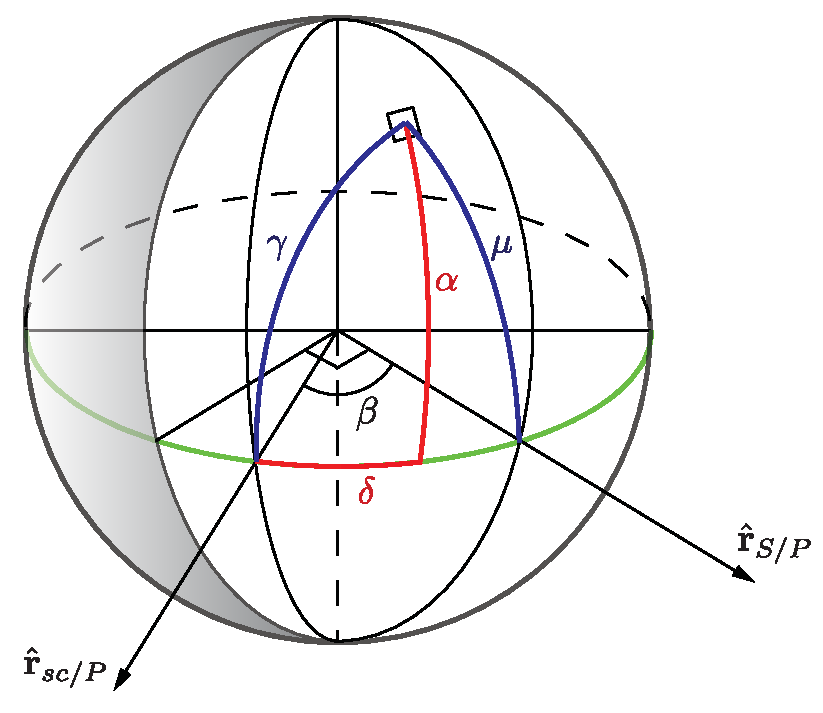
\includegraphics[height=160pt]{template/reflection_diagram}
}

\put(-10,205){\begin{minipage}[t]{0.6\linewidth}
\small{Energy per second per unit area per unit solid angle received by an observer =}
\vspace{-8pt}
\[ \frac{F R^2}{r^2} \int_{\beta - \pi/2}^{\pi/2} \cos(\beta - \delta) \cos\delta \intd{\delta}  \int_{-\pi/2}^{\pi/2} \rho(C_\mu,C_\gamma,\xi) \cos^3 \alpha \intd{\alpha} \]
\end{minipage}}

\put(110,147){\begin{minipage}[t]{0.4\linewidth}
\small{For isotropic scattering, $\rho$ = constant}
\end{minipage}}
\put(130,150){\begin{minipage}[t]{0.2\linewidth}
\[ \Phi(\beta) = \frac{E(\beta)}{E(0)} =  \]
\end{minipage}}

\put(160,120){\begin{minipage}[t]{0.2\linewidth}\
\[\frac{\sin(\beta)+(\pi-\beta)\cos(\beta)}{\pi} \]
\end{minipage}}

\put(170,90){\begin{minipage}[t]{0.2\linewidth}\
\[\frac{F_p}{F_S} = p\Phi(\beta) \left(\frac{R}{r}\right)^2\]
\end{minipage}}

\end{picture}
}

\section{Conclusions}
\subsection{Conclusions}
\frame{
\frametitle{Conclusions}
In conclusion: Don't forget your conclusions!
}

%let's make an appendix with refs and backup slides
%we don't want to count these in the slide total, so we'll stop counting here
\newcounter{finalframe}
\setcounter{finalframe}{\value{framenumber}}

\appendix

{
\subsection{References}
\frame[allowframebreaks]{
\frametitle{References}
\printbibliography  
}}

%backup slides:
\section{Backup}
\subsection{Backup}

\frame[label=backup1]{
\frametitle{A Backup Slide with Additional Info}
\framesubtitle{ \hyperlink{mainslide1}{\beamerreturnbutton{Return}} }
Lots of nitty-gritty stuff that doesn't belong in the main talk
}


\setcounter{framenumber}{\value{finalframe}} %reset the counter

\end{document}
